\subsection{The state of the art in theoretical frameworks for dark matter}
\label{sub:stateOfTheArtTheory}
\smallskip
%CD: The idea is not to have two separate DM and theoretical framework sections, but rather have everything in ~1 page with much sharper concepts (AB comment "misses the point" had a point).  

%Aims of this paragraph: DM and why should we look for it at the LHC
Gravitational and cosmological observations~\cite{Bertone:2016nfn} point to the existence of dark matter, for which the SM does not provide any explanation. 
Many extensions to the SM explain the present amount of dark matter in our universe (called \textit{relic density}) by a connection to SM particles~\cite{Hall:2009bx,Bernal:2017kxu,Steigman:2012nb}~\footnote{Alternative explanations for DM exist, e.g.~\cite{McGaugh_2016,Lennon:2017tqq,Bird:2016dcv,Marsh:2015xka}. Given our ignorance on the genesis of DM, WP5 pursues a broad theoretical and experimental approach that considers different possibilities.}. 
%[CD: am I digging myself a hole? Also using the word genesis is not ideal. Also is a fun read: http://inspirehep.net/record/1711655] 

%Aims of this paragraph: introduce the WIMP and complementarity between ID/DD/LHC
A popular DM candidate satisfying the relic density is the WIMP, a TeV-scale stable particle with interaction strength comparable to the weak force.  
WIMPs are detectable by a variety of experiments. 
Indirect detection experiments (ID) could observe excesses of SM particles over astrophysical backgrounds due to WIMP annihilation in DM-rich regions~\cite{Gaskins:2016cha}. 
Direct detection experiments (DD) could detect the interaction between incoming WIMPs and recoiling target nuclei within the detector~\cite{Schumann:2019eaa}. 
Colliders such as the LHC could produce DM from collisions of SM particles in controlled conditions, allowing thorough exploration of DM-SM interactions. 
Detections in all three types~\footnote{Particles that look like DM to LHC experiments may decay after leaving the detector, with a lifetime incompatible with DM’s cosmological timescales.} are needed to obtain crucial complementary information on the physics of WIMP dark matter. 
\\
Exploiting this \textbf{synergy between different experiments} requires a well-specified \textbf{common theoretical ground}. 
%Aims of this paragraph: introduce simplified models, introduce Z' and its parameters, justify their use (too many aims?)
WIMP models range from ful theories such as supersymmetry (SUSY)~\cite{Martin:1997ns} to effective field theories (EFT) where at LHC energy scales the details of the interaction can be ignored~\cite{Goodman:2010ku}. 
During the course of my StG, I co-led the Dark Matter Working Group and produced the most widely-used, state-of-the-art for benchmark models for generic LHC DM searches~\cite{Abercrombie:2015wmb}. 
These focused experimental effort on \textbf{simplified models} that reduce a large number of theories to their basic LHC experimental features using the fewest possible model parameters. 
The simplified models introduce a new particle mediating the interaction between SM and DM particles. 
These mediators were a spin-1 particle analogous to the Z boson (a $Z’$ boson)~\cite{Shoemaker:2011vi,Buchmueller:2013dya,Chala:2015ama}, a new spin-0 scalar much like a new Higgs boson~\cite{Buckley:2014fba,Egana-Ugrinovic:2019dqu,Abe:2018bpo}, or a spin-2 graviton~\cite{Kang:2020huh}. 
%Here I want to show completeness
Models including a vector or scalar mediator have been used to benchmark the sensitivity of future facilities and compare them to the next-generation DD and ID experiments, by certain DD and ID experiments and as input to the update of the European Strategy of Particle Physics~\cite{Strategy:2019vxc}.
This complementarity of DD, ID and LHC experiments~\cite{Bauer:2013ihz} is fully rooted in the LHC DM search program as established during the course of my StG~\cite{Boveia:2016mrp}.
\\
While additional interactions and modifications are required to make simplified models self-consistent theories (see e.g.~\cite{Ellis:2018xal}), the modifications do not change an important experimental feature: detection of a signal in one type of DM search would imply an effective coupling between SM and DM particles that leads signals at the LHC of both invisible (imbalanced) decays and also visible decays into SM particles. 
Sensitivity to these visible decays gives LHC experiments unique capabilities to explore these dark interactions.
A discovery of DM in gamma ray observations should be followed by characterizing the mediator of its interactions at the LHC.
An LHC discovery of a mediator particle, when combined with relic density measurements, would focus non-collider searches on particular regions of DM masses and cross-sections.

\begin{wrapfigure}{R}{0.65\textwidth} 
\begin{center}
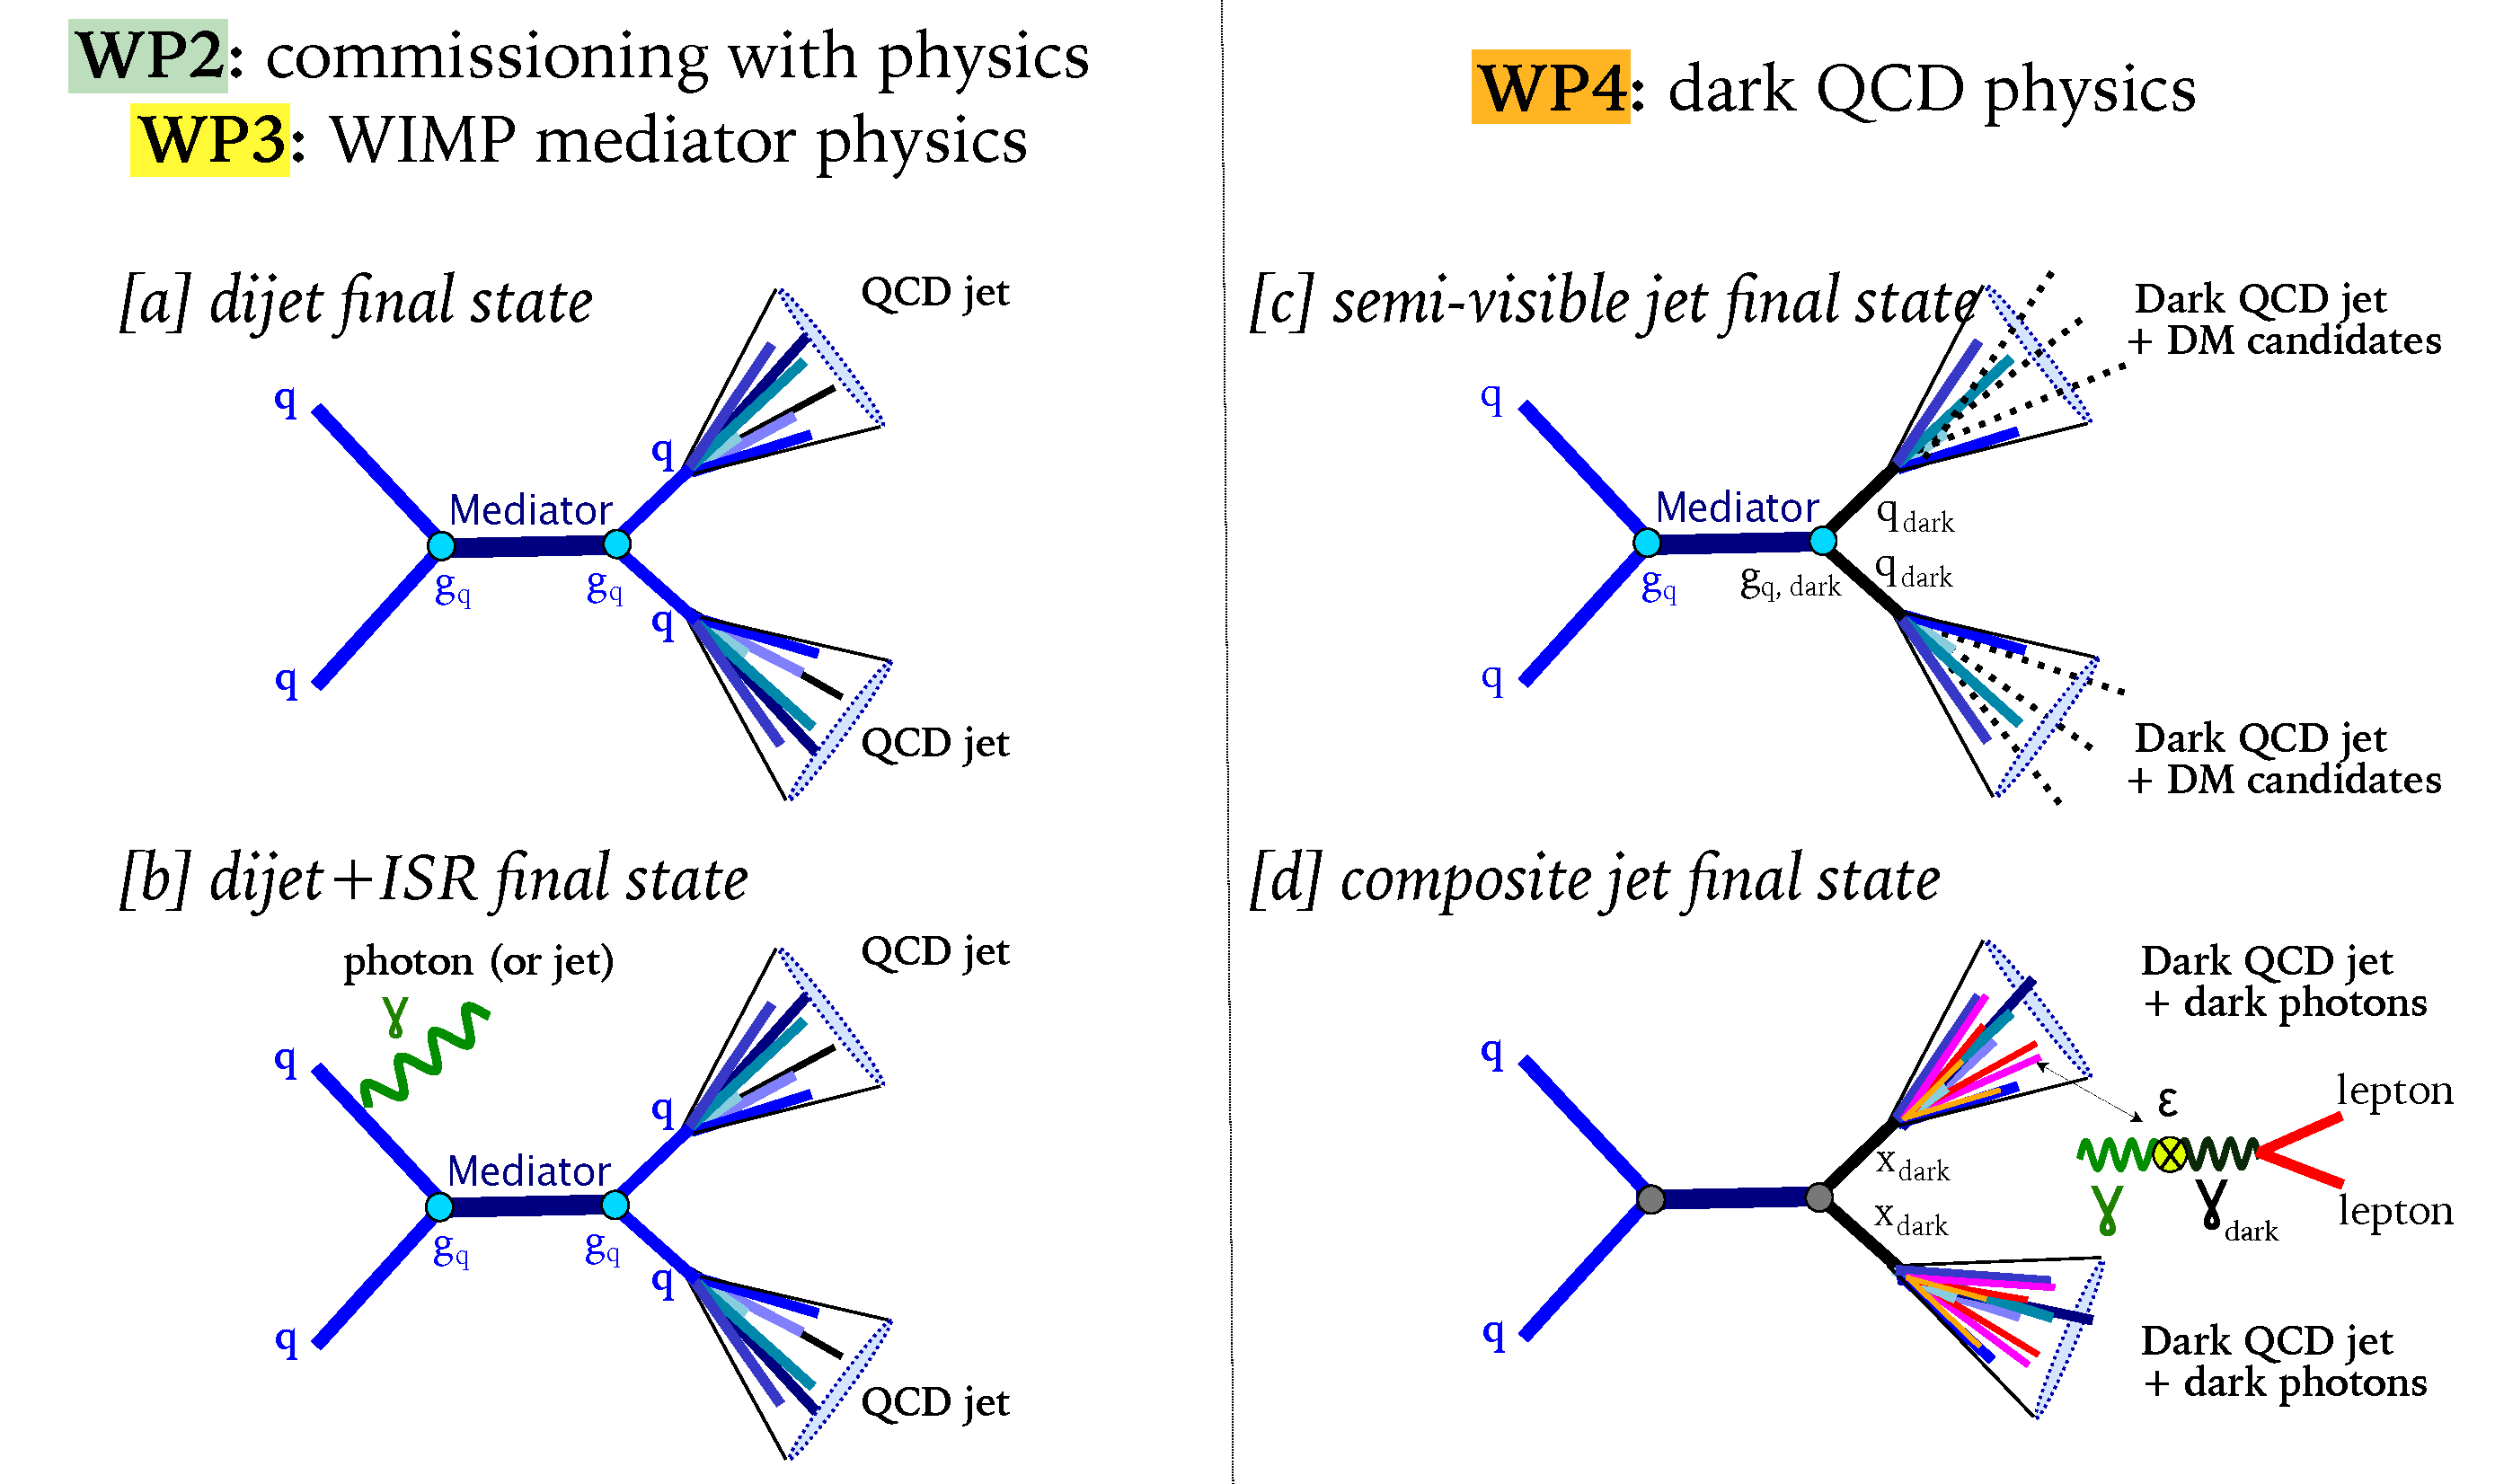
\includegraphics[width=0.65\textwidth]{figs_B2/feynman.pdf}
\caption{Sketches of search signatures in this project.\color{black}\label{fig:feynman} }
\end{center}
\vskip-10pt
\end{wrapfigure}
%\vskip5pt

Simplified models allow for a systematic exploration of LHC search targets by scanning the parameter space (DM mass $m_{DM}$, mediator spin and mass $m_{Med}$, couplings to DM $g_{DM}$ and SM $g_{SM}$).
Exploration of yet unprobed parameter space for mediator decays as in the left-hand side of Fig.~\ref{fig:feynman} motivates the searches in WP2 and WP3. 

%More to defend simplified models, maybe too much?
%Furthermore, motivating searches for only a handful of new particles with simple interactions even if they are part of a complex spectrum is conceptually supported by how ordinary particles were uncovered in the history of the SM: the first particles discovered were the most common ones, and further complexity was unraveled at a later date. 
%These searches will be used to commission trigger improvements in WP2-3 will improve  much greater sensitivity with respect to previous searches , and employ simplified models as building blocks for more complex theories (WP4). 

%Aims of this paragraph: introduce dark sector models and hidden sector
In parallel to WIMP searches, it is also imperative to \textbf{consider alternative DM signals that could have escaped detection}. 
Example models include mediator-like particles that do not directly connect DM and SM, but rather provide a \textbf{hidden portal} with much weaker interactions between a more complex dark sector and SM particles~\cite{Strassler:2006im}. 
\\
The symmetries of the SM can be used as guiding principle to construct the particle spectrum and the interactions of the new dark sector. 
A \textbf{new U(1) symmetry} introduces a portal particle called \textit{dark photon}~\cite{Holdom:1985ag,Curtin:2014cca}.   
The dark photon mixes with the ordinary photon, leading to rare but observable signatures from its decays to SM particles. 
This model is currently used as a benchmark for many high-intensity experiments and for future facilities~\cite{Strategy:2019vxc}. 
%Why according to Shaposhnikov (who motivated benchmarks): doesn't quite convince me. 
%Light particles have become a more popular search target because they can be used to solve particle physics  
%g-2, only in connection with DM
%and astrophysics anomalies 
%Pamela (bleurgh)
%too-big-to-fail as opposed to WIMPs - self-interactions
Models with a \textbf{new SU(2)}, also termed \textit{dark QCD} models for their similarity with SM QCD, predict fundamental components (dark quarks, $q_{dark}$) that are confined at an energy scale comparable to that of QCD~\cite{Bai:2013xga}. 
This leads to signatures of highly collimated particles, resembling hadronic jets that include dark sector particles and their decay products (\textit{dark jets}). 
\\
Concrete models realizing one or more dark QCD symmetries include asymmetric DM~\cite{Zurek:2013wia}, electroweak SUSY models~\cite{Cheung:2009su}, self-interacting DM~\cite{Tulin:2017ara}, and strongly-interacting DM~\cite{Bernreuther:2019pfb}). 
The large number of parameters and particles, and their subsequent variety of experimental signals, mandates \textbf{signature-driven searches} rather than searches targeting any specific theory. 
For this reason, the data-taking techniques in this project are designed to \textbf{record data that could contain multiple signatures, and that would otherwise be lost}. The searches in WP4, using the dark jets signatures shown in the right-hand side of Fig.~\ref{fig:feynman} \textbf{target two uncovered dark sector signatures} as representative use cases for this dataset. As shown in the right-hand side of Fig.~\ref{fig:feynman}, we will first search for dark jets containing thermal relic DM particles (semi-visible jets) produced from the decay of a $Z’$~\cite{Bernreuther:2019pfb,Cohen:2017pzm}, and subsequently for dark jets where the showering process interleaves dark photons and dark hadrons, leading to hadronic jets with an anomalous leptonic content (composite jets)~\cite{Cheung:2009su,Park:2017rfb}.
%Further thoughts are in here
%%Together or individually, mediator particles above and dark photons can also be part of a dark sector set of particles that do not interact significantly with the SM, including the DM candidate~\cite{Felix}. 

%Another possible story (but longer)
%Building blocks: dark QED
%Why attractive
%Conceptual connection to vector mediator above
%Why neglected
%Next-on: dark QCD
%Why attractive
%Why neglected




%For this reason, systematic exploration of these models does not proceed by scanning the theory’s parameter space, but rather by mapping the characteristics of different possible configurations of parameters and ensuring that no experimental stone is left unturned. 
%Searches for this kind of models have recently started taking shape at the LHC, in parallel to a vigorous pursuit by planned and existing non-LHC experiments~\cite{PBC}. 



%DM can't catch light DM even though there are a lot of tries
%So we go after the mediators again

%- Large experimental variability
%- Many motivations for lepton-jet models, but they neglect hadronic dark sector particles (eg SUSY lepton-jets below)
%- So we start where we can, and where we have motivations - B-L? 

%Peter's suggestion for B1, but I don't know where to add it? 
%The only thing I miss and I can understand that it can be hard to fit in is a motivation of WIMPs and
%in particular dark QCD. Could one maybe add just a little a la:
%The nature of dark matter is difficult to understand, because even today there is five times more
%dark matter than normal matter, this is only after essentially all normal matter in the Universe
%annihilated microseconds after the Big Bang (only 1 in 10,000,000,000 protons survived). The WIMP
%solution is a weakly coupled particle that yields the observed DM abundances by being weakly
%produced. It is attractive to search for WIMPs at the LHC because the energy of the accelerator
%allows studies above and below the electroweak phase transition. In Dark QCD one instead assumes that
%the abundances are similar because there also was an annihilation in the dark sector of the Universe
%and so Dark QCD models can potentially also explain the matter-antimatter symmetry observed in the
%Universe. It is attractive to search for Dark QCD at the LHC because it is a QCD collider and so one
%could expect that if there is a coupling between QCD and Dark QCD then we are likely to produce Dark
%QCD mesons and baryons at the LHC.%Check the latter

%SUSY lepton-jets: https://arxiv.org/pdf/0909.0290.pdf
%The cascades to N ̃1 may also result in colored particles and hence QCD-jets, but for the purpose of the current study we will assume that a substantial fraction of such cascades result in no colored particles. This is not a strong assumption as it is satisfied in many concrete examples of MSSM spectra [11], and may even be discarded altogether in actual lepton jet searches including QCD-jets.

%Existing text
%, and as a consequence it is only extremely feebly connected to electrically charged particles - I should probably talk about its decays
%too ambiguous? it decays into fermions as if it were a photon
%rather than direct interactions with


%This is one of the cases in which simplified models are used as building blocks for more complex models.


%In WP4, I will make use of my expertise in the reconstruction of hadronic jets and non-standard data taking technique to search for two classes of theoretically-motivated DM models that include a new strong force within the dark sector (dark QCD), using novel data taking techniques necessary for uncovering their signatures. 
%With these searches, this proposal will contribute to the systematic mapping of the territory of hidden sector signature, in synergy with other LHC and non-LHC searches. 

Depending on the SM-DM interaction strength and on the DM characteristics, a wealth of new experiments can contribute to the quest for WIMP and non-WIMP DM~\cite{Beacham:2019nyx,Bertone:2019irm,Barausse:2020rsu}.
There is a thriving scientific dialogue, with new ideas for DM and new ways to look for it continually emerging.
It is clear that, given the breadth of possible explanations for DM, an equally broad experimental and theoretical approach is needed, 
and new synergies can be exploited beyond the already-mentioned complementarity between DD/ID and colliders searches. 
This consideration inspires the work planned for WP5, taking place within newly established common platforms for dissemination of results and tools, in the spirit of open and collaborative science. 

\subsection{The state of the art in experimental tools for discovering dark matter and new phenomena}
\label{sub:stateOfTheArtExperiment}

\subsubsection{LHC and ATLAS: overview and schedule}
\smallskip

In 2021, after a period of upgrades expanding the discovery potential of ATLAS, the LHC will restart operations and continue delivering proton-proton collision data until the end of 2024. In this data-taking period (called \textit{Run-3}), up to 250/fb will delivered to the ATLAS experiment~\cite{ATLAS2008}.%{JINST2008}. 
It is expected that the bulk of the data will be collected in 2022 onwards, after commissioning the machine and the experiments in 2021. 

In Run-3, the LHC collision energy will not be increased significantly.
Absent anomalies in the Run-2 data~(189/fb), Run-3 will not grow the total dataset sufficiently to make new discoveries with its statistical power alone.
\textbf{New methods and technical innovations are required to discover rare processes}. %, mandates technical innovation.
Innovating the ATLAS data acquisition and selection system is an integral part of this project, 
as the key to extract a much larger amount of useful information from Run-3. 
This proposal is especially timely. The improvements within \textsc{Realdark} can be developed and tested with physics in early Run-3 data. 
Moreover, they must happen in advance of the LHC production phase to allow full exploitation of the Run-3 dataset. 

\subsubsection{The ATLAS trigger and its upgrades}
\smallskip

Recording all LHC collisions in ATLAS (up to 30 million collision events/second) is unfeasible due to storage and computing limitations. 
Therefore, most of the data are discarded before being analyzed in detail. \textbf{Only a small fraction of interesting events is selected} by the ATLAS trigger system. 
%The rest are discarded forever. 

The ATLAS trigger is composed of two levels~\cite{Aaboud:2016leb}. %2015TriggerPaper
The first hardware level (L1) performs an initial coarse selection within 2.5 $\mu s$, then 
passes collision eventws to the software-based High Level Trigger (HLT), implemented on a computing farm, where more sophisticated \textit{online} event reconstruction and data analysis are done. 
The HLT then decides to discard or keep the full detector information for the event.
Only if kept can further \textit{offline} reconstruction and analysis be done of electrons, muons, photons, jets, ... (called \textit{physics objects} in the following). 
The total event rate that can be retained after the HLT decision is directly \textbf{limited by the available output bandwidth and permanent storage}. 
%since traditional offline analysis currently requires the full set of detector information for reconstruction of physics objects (e.g. electrons, muons, photons, jets...). 
The rates of useful events recorded for offline analysis are also indirectly limited by the available HLT computing: 
a number of high-level features that would help in distinguishing signal from background are \textbf{too expensive to reconstruct given the available HLT resources}. 
%An example of such a feature is the track-collision vertex association for physics objects, 
%as this enables removing spurious contributions from simultaneous proton-proton collisions other the one of interest (pile-up). 
These limitations impairs the sensitivity of searches where signals are buried in high-rate backgrounds and motivates the improvements in WP1. 

For Run-3, the ATLAS trigger is undergoing significant upgrades~\cite{Aad:1602235}. 
The L1 trigger will be equipped with new electronic boards that allow for a more granular and efficient first decision. 
As part of my StG, my team has developed control software for the board which will permit using information from the entire hadronic calorimeter at once (gFEX)~\cite{Tang:2016ded}, 
and contributed software for the new jet board (jFEX)~\cite{Bauss:2018nde}. 
Furthermore, the HLT software is being rewritten in a multithreaded framework~\cite{Bielski:2674286}, and the increased size of the HLT farm will significantly increase its computing power.
Optimized algorithms\footnote{See Ref.~\cite{ATL-PHYS-PUB-2019-041} %Elsing 
for an example of the improvements from optimizing tracking algorithms on simulated data containing 200 simultaneous collisions for the ATLAS high luminosity upgrade}. 
and increased HLT capacity will make tracking information more widely available at the trigger level than during Run-2. 
The new tracking information will be crucial to reject backgrounds from simultaneous proton-proton interactions (pile-up) that would otherwise limit the reach of the DM searches in this project.
Moreover, the Run-3 upgrades to the trigger software make it possible, for the first time in ATLAS, to record objects reconstructed directly at the HLT simultaneously with raw detector information in select regions of interest, a technique called Partial Event Building or PEB that was previously restricted to muons calibration and $B$-physics. 
Testing and exploiting these upgrades is an integral part of this project. 

%Among those, a full overhaul of the electronic boards that read in calorimeter information is foreseen. 
%The board that reads information from the electromagnetic calorimeters (eFEX) will allow for more refined distinction between electrons and photons already at L1. 
%This motivates the implementation of alternative data-taking techniques to overcome these limitations, as proposed in WP1 and discussed in the next section. 
%This can probably be removed since I don't use it directly anywhere else? 

\subsubsection{Review of analysis strategies for DM and related particles at the LHC}

Traditionally, searches for \textbf{WIMP Dark Matter} at colliders seek excesses of events with a momentum imbalance, where weakly or non-interacting particles escape the detector unseen~\cite{Boveia:2018yeb}. 
However, as seen in Sec.~\ref{sub:stateOfTheArtTheory}, many signal models also have unavoidable fully-visible signatures, such as when a mediator decays into SM particles.
Thus, searches for visible decays of the mediators are complementary to searches for invisible particles~\cite{CMSSummary,ATLASSummary}.
%Another point to look for visible decays, but not relevant here: 
%Considering the simple picture of \textbf{Fig. X}, invisible signals will be suppressed with respect to visible signals if the DM particle is much heavier than the particle mediating the interaction and invisible decays must occur off-shell. 
%\textbf{Decide: dijet/di-jet}
%Searches for visible signatures is an established complementary alternative to searches for invisible particles, with different challenges and sensitivity~\cite{ToBeCited}.%Summary plots 
DM mediator searches in visible decays also connect naturally with well-known, more broadly-motivated searches for new resonances at particle colliders, driving interest in difficult regions of phase space not constrained by existing searches~\cite{Kim:2019rhy}.%{Craig2bodyResonances}
%\\
%\indent

The searches in WP2 and WP3 in this project focus on a broadly-motivated yet experimentally challenging category of decays (see e.g.~\cite{Chala:2015ama}). 
Having been produced via a quark-quark vertex, the mediator will also decay back into quarks (Fig.~\ref{fig:feynman} [a]). 
The signature of this process is a resonant peak in the two-jet (dijet) invariant mass, peaking atop the smooth QCD background.
%%The relatively low background rates of high-mass hadronically-decaying resonances permit collecting all events in full above a threshold of approximately 1 TeV~\cite{ToBeCited}. 
The challenge of this signature lies below 1 TeV, where large amounts of QCD backgrounds overwhelm the experiment’s data storage resources~\cite{Sirunyan:2019vgj,Aad:2019hjw}. %high-mass dijets  
For this reason, dijet resonances with masses at and just above the electroweak scale (from $\approx$100 to several hundred GeV) have been very difficult to probe with standard data-taking techniques. 
%\\
%\indent

Discovering \textbf{resonances with sub-TeV masses require novel data-taking techniques and/or targeted signatures}. 
%During my StG, my team and I have pursued both directions within ATLAS. 
Following the Data Scouting technique in CMS~\cite{Khachatryan:2016ecr} and the Turbo Stream in LHCb~\cite{Aaij:2016rxn}, my StG team and I prototyped the \textbf{Trigger Level Analysis (TLA) technique} for jets. 
In this technique, high-level jet information is retained for all dijet events reconstructed by the HLT, discarding raw data. 
This allows for for a much smaller event size and much higher event rates~\cite{Aaboud:2018fzt}.%TLA PRL 
%\\
%

In normal-luminosity data-taking conditions, TLA dijet searches are still limited to resonances with masses above 450 GeV by the L1 event rate. 
Other detector signatures with reduced background rates are used to reach lower mediator masses, albeit at the cost of reduced signal acceptance.
One such signature that my collaborators and I introduced to the LHC in Run-2 is the \textbf{dijet+ISR signature}~\cite{An:2012ue,Aaboud:2019zxd}. 
Here, the resonance recoils against a high-p$_{\rm{T}}$ photon or gluon radiated from the initial-state quarks (Fig.~\ref{fig:feynman}, [b]). 
The requirement of an energetic object at the HLT reduces the background and allows to reach lower mediator masses, 
but limits the signal acceptance. 
Lowering the threshold on the ISR objects would increase the mass coverage and signal acceptance.
This motivates combining the TLA technique for the dijet+ISR signature for the first time in ATLAS\footnote{The CMS search in Ref.~\cite{Sirunyan:2019pnb} %CMS dijet+ISR
combines the dijet+ISR signature with the Scouting technique, but it does not surpass the sensitivity of the offline ATLAS search as it is limited to a limited Run-2 dataset with special triggers.}, as planned for WP3. 
\\
Combined, ATLAS and CMS low-mass dijet resonance searches using the TLA/Scouting and dijet+ISR approaches~\cite{Aaboud:2018fzt,Sirunyan:2019pnb},
including searches targeting resonances decaying in heavy flavor quarks~\cite{EXOT-2016-33,CMS-EXO-16-057} %di-b 
and/or where the resonance is boosted~\cite{EXOT-2017-01,CMS-EXO-17-001,Sirunyan:2018ikr,ATLAS-CONF-2018-052,Sirunyan:2019vxa}, %CMS and ATLAS dijet ISR boosted, including di-b
improve coverage of the EW scale but fail to probe it to the degree required, or as thoroughly as at higher masses.

In the mass range where the weak force mediators reside, and that is favored in WIMP and non-WIMP $Z’$ models fitting ID excesses~\cite{Hooper:2019xss}m %Hooper&Leane  
these searches are only sensitive to coupling strengths well above those of the weak force or those probed by DD for a narrower set of signals.
Pushing the collider sensitivity in this region will help validate and characterize a possible DM interpretation of DD results~\cite{Ellis:2018xal,Kang:2020huh,Alves:2016cqf} and open it to discovery of DM signals beyond those probed by DD.

\begin{wrapfigure}{R}{0.5\textwidth} 
\begin{center}
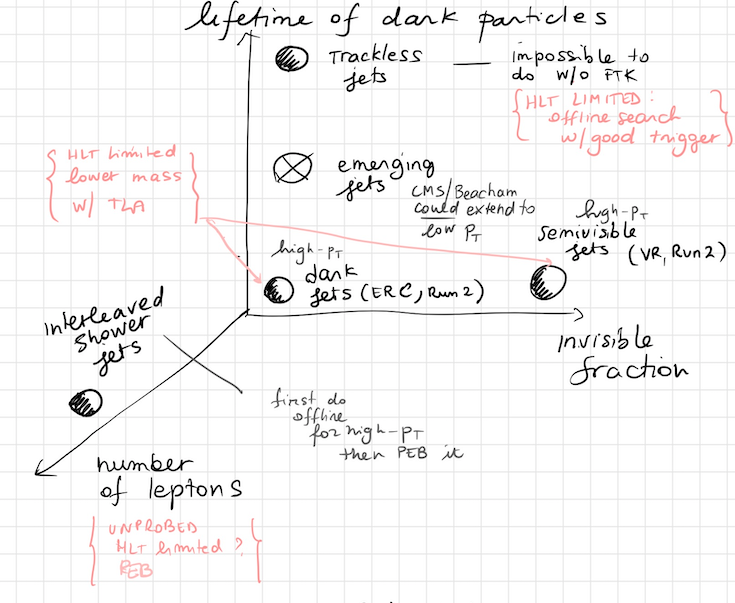
\includegraphics[width=0.5\textwidth]{figs_B2/DarkSectorSketch}
\caption{Sketches of covered and uncovered search signatures for dark jets. This sketch does not include searches for individual components of the dark jets. \label{fig:darksectorssketch} }
\vskip-10pt
\end{center}
\end{wrapfigure}
%Alternative text because Dark QCD is sometimes strongly interacting?
%Partly motivated by the constraints set on such particles by first-generation direct searches and by results obtained in the first phase of the LHC data-taking, the DM community has recently started to generalize the flagship searches for these weakly interacting massive particles (WIMPs) by expanding the search program for particles with either stronger or much weaker interactions with SM particles than what predicted by WIMP theories~\cite{FIMPs, StronglyInteracting}, or much lighter particles~\cite{DarkPhotons, ALPs}, or much more massive objects (e.g. Primordial Black Holes)~\cite{GW paper}~\footnote{Such scenarios can also fit the measurements of the relic density of dark matter through different mechanisms~\cite{FreezeIn}}. 
 
DM mediators inspired by the EW sector have a well-mapped landscape, though it is not yet fully constrained.
The state-of-the-art of \textbf{hidden sector and dark QCD searches}, however, leaves much room for both experimental and theoretical improvement.
Hidden sector models generally imply more difficult detector signatures than considered here so far. 
Examples of these signatures are particles with a long lifetime that decay far from the interaction point.
These are not suited to standard reconstruction techniques~\cite{Lee:2018pag} and their most distinctive features, such as displaced decays or unexpected particles within the busy environment of a hadronic jet, are too expensive to reconstruct at the HLT. %DRAW
This forces searches to rely on triggers that let large amounts of background through (e.g. missing transverse energy or purely hadronic triggers) and consequently induce limitations on what kinematic regions can be searched, or force triggering in less general, more model-dependent ways. 
With the TLA+PEB technique, however, more complex features can be reconstructed after only a coarse preselection, limiting the loss of search generality. In TLA+PEB, the event size is reduced with respect to traditional data analysis, so that the signal rates recorded can be increased. 
 % with a small enough event size and increased signal rates with respect to traditional searches.%, limiting the loss of generality of the search. 

To search broadly for such models, we will employ a signature-driven rather than model-driven approach.
% for choosing and designing Run-3 searches to be performed using this technique within the timeframe of this proposal 
As specified in Sec.~\ref{sub:stateOfTheArtTheory}, we adopt the grounding assumption that the confinement scale is sufficient to produce dark jets. 
 %Ohm Soffer review 
As an initial guide to the experimental state-of-the-art for the searches in WP4, dark jets can be classified according to their main features. 
Extending Ref.~\cite{Cohen:2017pzm,Park:2017rfb}, Fig.~\ref{fig:darksectorssketch} characterizes dark jets according to the following.  
\\
\indent
\textbf{1.} Depending on how many of the constituents of the the dark jet are long-lived, the dark jet will appear in the detector at different distances with respect to the interaction point. ATLAS and CMS searches pursue these signatures, looking for \textit{emerging}~\cite{Schwaller:2015gea,Sirunyan:2018njd}, \textit{displaced} or {trackless jets}~\cite{Aaboud:2019opc,Sirunyan:2018vlw,DeBruyn:2018cdo} jets and for the long-lived particles themselves (e.g.\cite{Sirunyan:2019nfw}, for a review, see Ref.~\cite{Lee:2018pag}). Together with colleagues from LPSC Grenoble and Witswatersrand, I am pursuing the first-ever LHC search for signatures of jets whose constituents are prompt and fully visible but fragment differently (\textit{prompt dark jets})~\cite{Park:2017rfb}, with a publication expected by Fall 2020. 
\\
\indent
\textbf{2.} The dark jet may be constituted by a sizable fraction of invisible particles, e.g. stable dark sector particles and DM candidates, and appear as a \textit{semi-visible dark jet}. In this case, we assume that the lightest particles in the dark sector are the DM candidates following Refs.~\cite{Cohen:2017pzm,Park:2017rfb,Bernreuther:2019pfb}\footnote{Dark sector / dark pion decays into SM particles motivate other searches that will be connected to the ones in this project within WP4/5, for example emerging/trackless jets and searches in the review of Ref.~\cite{Kribs:2018ilo}}.%Kribs, https://lhcbproject.web.cern.ch/lhcbproject/Publications/LHCbProjectPublic/LHCb-PAPER-2016-065.html
\\
\indent
\textbf{3.}  The dark jet may contain an unusual number of leptons from leptonically-decaying dark photons. Jets composed exclusively of leptons (lepton-jets) are covered by ATLAS and CMS searches~\cite{Aad:2019tua,EXOT-2014-09,Khachatryan:2015wka}, %ATLAS long lived LJ: Aad:2019tua, ATLAS prompt LJ: EXOT-2014-09
but mixed cases of hadrons and muons are only partially covered as many searches apply an isolation requirement to leptons~\footnote{Ref.~\cite{Chatrchyan:2011hr} searches for muon pairs without isolation, only using a small amount of Run-1 data, while \cite{Sirunyan:2019wqq} searches for dark photons to dimuons without an isolation requirement, starting at dark photon masses above 10 GeV}. %LeptonJets

From this classification, \textbf{Semi-visible jets}  (Fig.~\ref{fig:feynman} [c]) are experimentally uncovered at the time of writing. 
%Should I say this? 
%~\footnote{I am involved in an ongoing search for semi-visible jets in ATLAS and CMS with Run-2 data, but the benchmarks used and mass range are different to those used in this proposal. There is also an ongoing CMS search using Run-2 data.}.
Similarly, \textbf{composite jets} where dark QCD and dark photon showers are interleaved producing a cascade of a variable number of leptons and hadrons within the same jet (Fig.~\ref{fig:feynman} [d]) have not been sought at the LHC before. 
This motivates the choice of the two WP4 searches. 

Experimental attention generally stimulates theoretical development and extensions of unprobed models, as well as efforts towards their systematic classification. 
As part of WP5 in this project, we will organize workshops and open a number of discussion channels with the theory, astroparticle, non-collider and nuclear physics communities. 
This cross-talk will be useful for input on search targets, on the simulation of benchmark models and for the contextualization of search results.
